%
% uebersicht.tex -- Uebersicht ueber die Seminar-Arbeiten
%
% (c) 2022 Prof Dr Andreas Mueller, OST Ostschweizer Fachhochschule
%
\chapter*{Übersicht}
\fancyhead[RE]{}
\fancyhead[LO]{Übersicht}
\label{buch:uebersicht}
Im zweiten Teil kommen die Teilnehmer des Seminars selbst zu Wort.
Die im ersten Teil dargelegten mathematischen Methoden und
grundlegenden Modelle werden dabei verfeinert, verallgemeinert
und auch numerisch überprüft.

Die Lagrange-Mechanik kann die Herleitung von Bewegungsgleichungen
in komplizierten mechanischen Systemen stark vereinfachen.
\textit{Shaarujan Kamalanathan} führt dies am Beispiel des
Doppelpendels durch.
Seine Simulation zeigt auch das chaotische Verhalten des Doppelpendels.

Ein klassische Anwendung der Variationsrechnung ist die Bestimmung
der Kurve, der eine frei hängende Kette folgt.
\textit{Tobias Locher} und \textit{Nico Tuscano}
führen die Rechnung durch, illustrieren sie aber auch durch schöne
eigene Experimente.

Die Kettenlinie tritt auch als Merdiankurve einer Rotationsfläche
minimalen Inhalts auf.
\textit{Ronja Allenfort} und \textit{Ana Milivojevic} führen in die
Theorie der Minimalflächen ein und zeigen, dass das Katenoid,
die Rotationsfläche der Kettenlinie, minimalen Flächeninhalt hat.
Die beiden Autorinnen haben auch ein Katenoid als Seifenhaut
realisiert und damit das Umschlagbild dieses Buches beigesteuert.

Die Mechanik der Massepunkte lässt sich aus Variationsprinzipien
herleiten.
\textit{Sofia Aaltonen} und \textit{Gabriella Rodrigues} zeigen
am Beispiel der Balkengleichung, dass dies auch für die elastische 
Verformung von Körpern gilt.

Noch komplexer als die Mechanik der elastischen Körper ist die
Strömungsmechanik.
\textit{Sven Schlömmer} zeigt, wie man aus einem Variationsprinzip,
der Lagrange-Funktion von Luke, eine partielle Differentialgleichung
für nichtlineare Oberflächenwasserwellen, die Saint-Venant-Gleichung,
bekommen kann.

Die Anwendung von Variationsprinzipien ist nicht auf die
klassische Mechanik beschränkt.
\begin{figure}
\centering
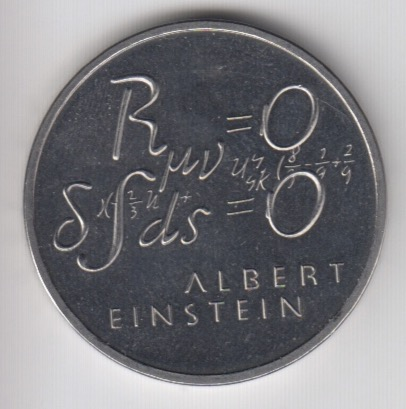
\includegraphics[width=5cm]{papers/Einstein5Fr.jpg}
\caption{Variationsprinzip der Relativitätstheorie auf dem
Gedenkfünfliber zum 100.~Geburtstag von Albert Einstein
aus dem Jahr 1979.
Die Bewegungsgleichungen der Relativitätstheorie lassen sich aus
dem Variationsproblen $\delta \int ds=0$ ableiten.
\label{buch:papers:fig:5liber}}
\end{figure}%
Auch in der relativistische Mechanik lassen sich die Bewegungsgleichungen
aus einem Variationsprinzip ableiten, welches man sogar auf
dem Gedenkfünfliber zum 100.~Geburtstag Albert Einsteins aus dem
Jahr 1975 finden kann (Abbildung~\ref{buch:papers:fig:5liber}).
\textit{Selvin Blöchlinger} leitet die relativistischen
Bewegungsgleichungen für ein geladenes Teilchen in einem
elektromagnetischen Feld ab.

Die Gleichungen des elektromagnetischen Feldes werden normalerweise
durch die Maxwell-Gleichungen beschrieben.
\textit{Maurin Doswald}
und
\textit{Stephan Oseghale}
leiten sie aus einem Variationsprinzip her.

Das Variationsprinzip, welches die relativistischen Bewegungsgleichungen
liefern, ist eigentlich ein Minimalproblem für die Kurvenlänge.
Solche Kurven heissen Geodäten.
\textit{Andrin Kälin}
und
\textit{Marco Rouge}
entwickeln den Formalismus der Geodätendifferentialgleichung aus
den Euler-Lagrange-Differentialgleichungen für die Kurvenlänge.

Auch für die Gleichungen, die das Verhalten elektrischer Ströme in 
einer Schaltung beschreiben, lässt sich ein Variationsprinzip 
finden.
Es ermöglicht, die Stromverteilung auch in kontinuierlich verteilten
Medien zu berechnen, wie dies \textit{Matthias Meyer} durchführt.

An der Schnittstelle zwischen einer Schaltung und dem elektromagnetischen
Feld steht jeweils eine Antenne.
\textit{Baris Catan}
und
\textit{Jannis Gull}
zeigen, wie man die Form einer Antenne mit dem Ritz-Verfahren,
einem direkten Verfahren der Variationsrechnung,
optimieren kann.

Schon Leonhard Euler hat sich mit der Frage befasst, wie man 
am schnellsten durch die Strömung eines Flusses schwimmt.
\textit{Anna Pietak} untersucht dieser Frage in Ihrer Arbeit.

Allgemeiner einsetzbar als das Ritz-Verfahren ist die Methode
der finiten Elemente, in die \textit{Flurin Brechbühler} einführt.

Ein besonders anspruchsvolles Minimalproblem ist die Aufgabe,
eine Nutzlast mit Hilfe einer Rakete in eine Erdumlaufbahn zu
bringen.
\textit{Joel Stohler}
und
\textit{David Peter}
zeigen, dass diese Aufgabe auf ein optimales Steuerungsproblem
führt.

Warum sind alle Planeten kugelförmig?
\textit{Jakob Gierer}
und 
\textit{Lukas Schöpf}
lösen das Problem des hydrostatischen Gleichgewichts und
zeigen so, dass die Form geringster Energie eine Kugel ist.

Der Begriff Variation wird auch für Algorithmen verwendet.
\textit{Kevin Kempf} führt in dieses Thema ein und stellt
einen Vergleich zur Variationsrechnung an.

Die Entmischung von Legierungen wird durch die Cahn-Hilliard-Gleichung
beschrieben.
\textit{Patrik Müller} stellt den unmittelbaren Praxisbezug her,
indem er nicht nur die Gleichung herleitet, sondern auch auf
das Problem anwendet, eine gute Salatsauce herzustellen.







